\documentclass{article}
\usepackage{amsmath}
\usepackage{fancyvrb}
\usepackage{amssymb}
\usepackage{amsthm}
\usepackage[margin=0.8in]{geometry}
\usepackage{hyperref}
\usepackage{physics}
\usepackage{tikz}
\usepackage{mathtools}\mathtoolsset{showonlyrefs}
\usetikzlibrary{calc,positioning,shapes.geometric}
\tikzstyle{db} = [ 
	cylinder,
	cylinder uses custom fill,
	cylinder body fill = yellow!50,
	cylinder end fill = yellow!50,
	shape border rotate = 90,
	aspect = 0.25,
	draw
	]
\tikzstyle{serv} = [
	ellipse,
	fill = gray,
	draw
	]
\tikzstyle{daq} = [
	rectangle,
	aspect = 0.5,
	draw
	]

\tikzstyle{evlist} = [
	ellipse,
	draw
	]
\tikzstyle{data} = [
	->,
	thick,
	red,
	draw
	]
\tikzstyle{bidir} = [
	<->,
	dashed, thick, draw
	]
\author{Connor Duncan}
\date{\today}
\title{\texttt{tesdaq} Redis Message Documentation}
\setlength\parindent{0pt}


\begin{document}
\maketitle
\tableofcontents

\section{Introduction}
This document exists to help standardize and explain how messages are sent via Redis when functions like \texttt{DAQCommander.start(**kwargs)} are called. It will begin with a basic overview of the structure of the application, before explaining how commands are sent, and configurations recieved, before finally discussing the format in which data acquired is sent to the server and ultimately the client.

This document will mention \texttt{adcscope}\footnote{the server developed as the frontend/pulseviewer} several times as well, but will hopefully provide examples and instruction of how to extend the functionality of this library to any DAQ system.
\subsection{Application Structure}
First, the application consists of essentially two types of program. There are listeners, and commanders. The name commanders is derived from the fact that these issue commands to the listeners.
This uses a Redis database to facilitate communication between the various programs, with several functions that extract information from messages posted in the database.

\begin{center}
	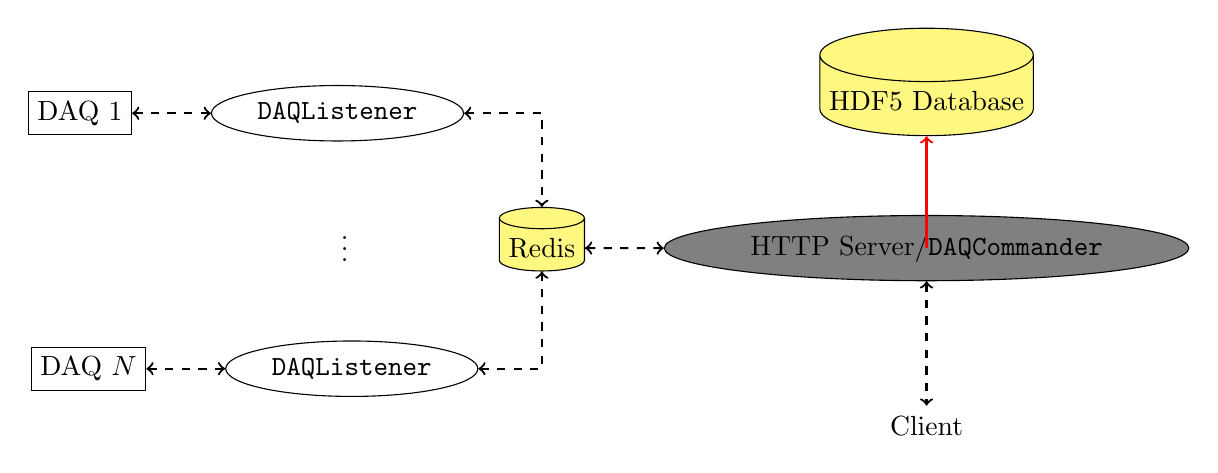
\begin{tikzpicture}
		\node[db] (rdb) at (0,0) {Redis };
		\node[serv, right=of rdb] (serv){HTTP Server/\texttt{DAQCommander}};
		\node[db,above =of serv] (h5) {HDF5 Database};
		\node[evlist, below left=of rdb] (e2) {\texttt{DAQListener}};
		\node[evlist, above left=of rdb] (e1) {\texttt{DAQListener}};
		\path (e2) -- node[auto=false]{\vdots} (e1);
		\node[daq,left=of e2] (d2) {DAQ $N$};
		\node[daq,left=of e1] (d1) {DAQ 1};
		\draw[bidir] (e2)--(d2);
		\draw[bidir] (e1)--(d1);
		\draw[bidir] (e2)-|(rdb);\draw[bidir](e1) -| (rdb);
		\draw[bidir] (rdb) -- (serv);
		\draw[data] (serv) -| (h5);
		\draw[bidir] (serv) -- ++(0,-2) node[anchor=north] (c) {Client};
	\end{tikzpicture}
\end{center}
Bidirectional arrows indicate data can both be transferred and return from each connected node, while a unidirectional arrow indicates data can only be transferred in one direction. 
Essentially, because the flask server already sits in an \texttt{event()} loop, it serves the role of listening for commands from the Redis Database (especially configuration, which is only read when a client pulls up the configuration pane containing a specific DAQ). 
This will be explained more later in the discussion of \texttt{flask\_socketio}.


\section{Commands}


\section{Device Configuration}
\subsection{In-Redis Store of Config}
This is likely the most important section. My plan for storing data within the redis database revolves around using it's \texttt{SET} and \texttt{GET} capabilities to store the current allowable settings of the device, as well as whether or not it is running.

Currently, the only devices I am working with are National Instrument's PCI cards, so I will use that as my template.
Since each DAQListener should only correspond to one device, whenever it starts up, it should have some config file (or read parameters from the init method), which it then posts to the RDB. This should be a JSON string that has the following parameters:
\begin{Verbatim}[tabsize=4]
device = { # in this case device should be the **name** of the device (i.e. what you call it in Redis) 
	channel_type:	{	# e.g. "Analog Input" or "ai_in"
		channels: ["Dev1/ai0",...], # physical names of channels corresponding to input functions
		max_sample_rate: some_large_int,
		min_sample_rate: some_small_int,
		sr_is_per_chan:	False, # means if max sr is 800kS/s, with two channels, each can do 400 kS/s
		trigger_opts: [] # string values correspond to functions on each channel.
		},
	is_currently_running: False
}
\end{Verbatim}
Eventually, there will be a function that creates this string for you out of the parameters passed to your extension of \texttt{DAQListener}, which should make this fairly straightforward.
Then, what will happen, is when the \texttt{DAQListener} starts, it will use the \texttt{redis.SET} function to have the value corresponding to key \texttt{device} be set to the JSON object.
Whenever a client connects to the config page, the redis database will be queried for all currently available devices on the system, and whenever devices are selected, these parameters will be read into a form that will automatically try to validate and constrict the user to not do things that might otherwise break the DAQ.

This is a fairly limited code pattern, so more features will probably be added in the future. It's also easy to extend this feature to provide custom functions/restrictions, but that will require you to write a frontend for the form, which is what I want to prevent in the first place.

Also, if the variable \texttt{is\_currently\_running} doesn't exist, the Redis database should block all commands issued to that channel (because you don't want to accidentally run two tasks on a card at once).

\subsection{Why this is better}
I chose to do it this way as opposed to use something like an SQL database to store this information for several reasons.
\begin{itemize}
	\item The admin already has to set up a Daemon for each DAQ. This fits well into the intended workflow of one-time setup of devices, by configuring the constraints in advance.\footnote{Persistent configurations of devices is another bridge we will cross later.}
			\item SQL is annoying when you don't have permissions to edit files on servers (which is the case in many large confluences).
			\item Redis is substantially faster, and this also reduces the number of unique requests the HTTP server needs to make, because the messages can be packed into one long string, reducing network latency.
\end{itemize}

\section{Data}

\end{document}
